\documentclass{beamer}
\usepackage[utf8]{inputenc}
\usepackage{graphicx}

\hypersetup{
    colorlinks,%
    citecolor=blue,%
    filecolor=blue,%
    linkcolor=blue,%
    urlcolor=blue 
    %urlcolor=mygreylink     % can put red here to better visualize the links
}

\author[Sowmya Vajjala]{Instructor: Sowmya Vajjala}

\title[LING 520]{LING 520: Computational Analysis of English}
\subtitle{Semester: FALL '16}

\date{27 October 2016}

\institute{Iowa State University, USA}
%%%%%%%%%%%%%%%%%%%%%%%%%%%

\begin{document}

\begin{frame}\titlepage
\end{frame}

\begin{frame}
\frametitle{Class Outline}
\begin{itemize}
\item Reminder: Assignment 4 submission due on Saturday
\item Comment: The dictionary saving example I showed -  is just one simple way of doing it. There are several other ways (e.g., using numpy library)
\item Today's topics:
\begin{itemize}
\item Natural language parsing: an introduction
\item NLTK exercises
\end{itemize}
\end{itemize}
\end{frame}

\begin{frame}
\frametitle{}
\Large Natural Language Parsing - Introduction
\end{frame}

\begin{frame}
\frametitle{What is parsing?}
\begin{itemize}
\item In the context of NLP, parsing refers to converting a sentence into some form of syntactic structure.
\item syntactic structure includes: grammatical relations (subject-object etc), grouping constituents together (NP, VP etc), governor-dependent relationships etc.
\end{itemize}
\end{frame}

\begin{frame}
\frametitle{Why parse at all?}
\begin{itemize}
\item Can you think of some reasons to parse the syntactic structure? Where is it useful? \pause
\item Some imaginary examples where parsing the syntax is useful:
\begin{enumerate}
\item You may want to study how certain grammatical structures are used in applied linguistics vs biology research articles
\item or how Arabic L1 people write English compared to Chinese L1, but beyond simple vocabulary based patterns. \pause
\item You may want to design a system to understand the meaning of a sentence (automatically). Why? 
\item You may want to extract 'who did what to whom' kind of information automatically from a novel. \pause 
\item Although ngrams and POS tags are relatively straight forward to extract, they cannot give you this information. 
\end{enumerate}
\end{itemize}
\end{frame}

\begin{frame}
\frametitle{How to parse?}
\begin{itemize}
\item Clearly, we need POS tags, but also something beyond them get this kind of information. 
\item There are two main ways to show syntactic structure in NLP: Constituency structure and Dependency structure. 
\item Constituency structure shows the sentence as relations between its constituents (phrases), based on a pre-defined grammar.
\item Dependency structure shows modifier-modified, argument relationships etc. between words. 
\end{itemize}
\end{frame}

\begin{frame}
\frametitle{Examples of parsed sentences}
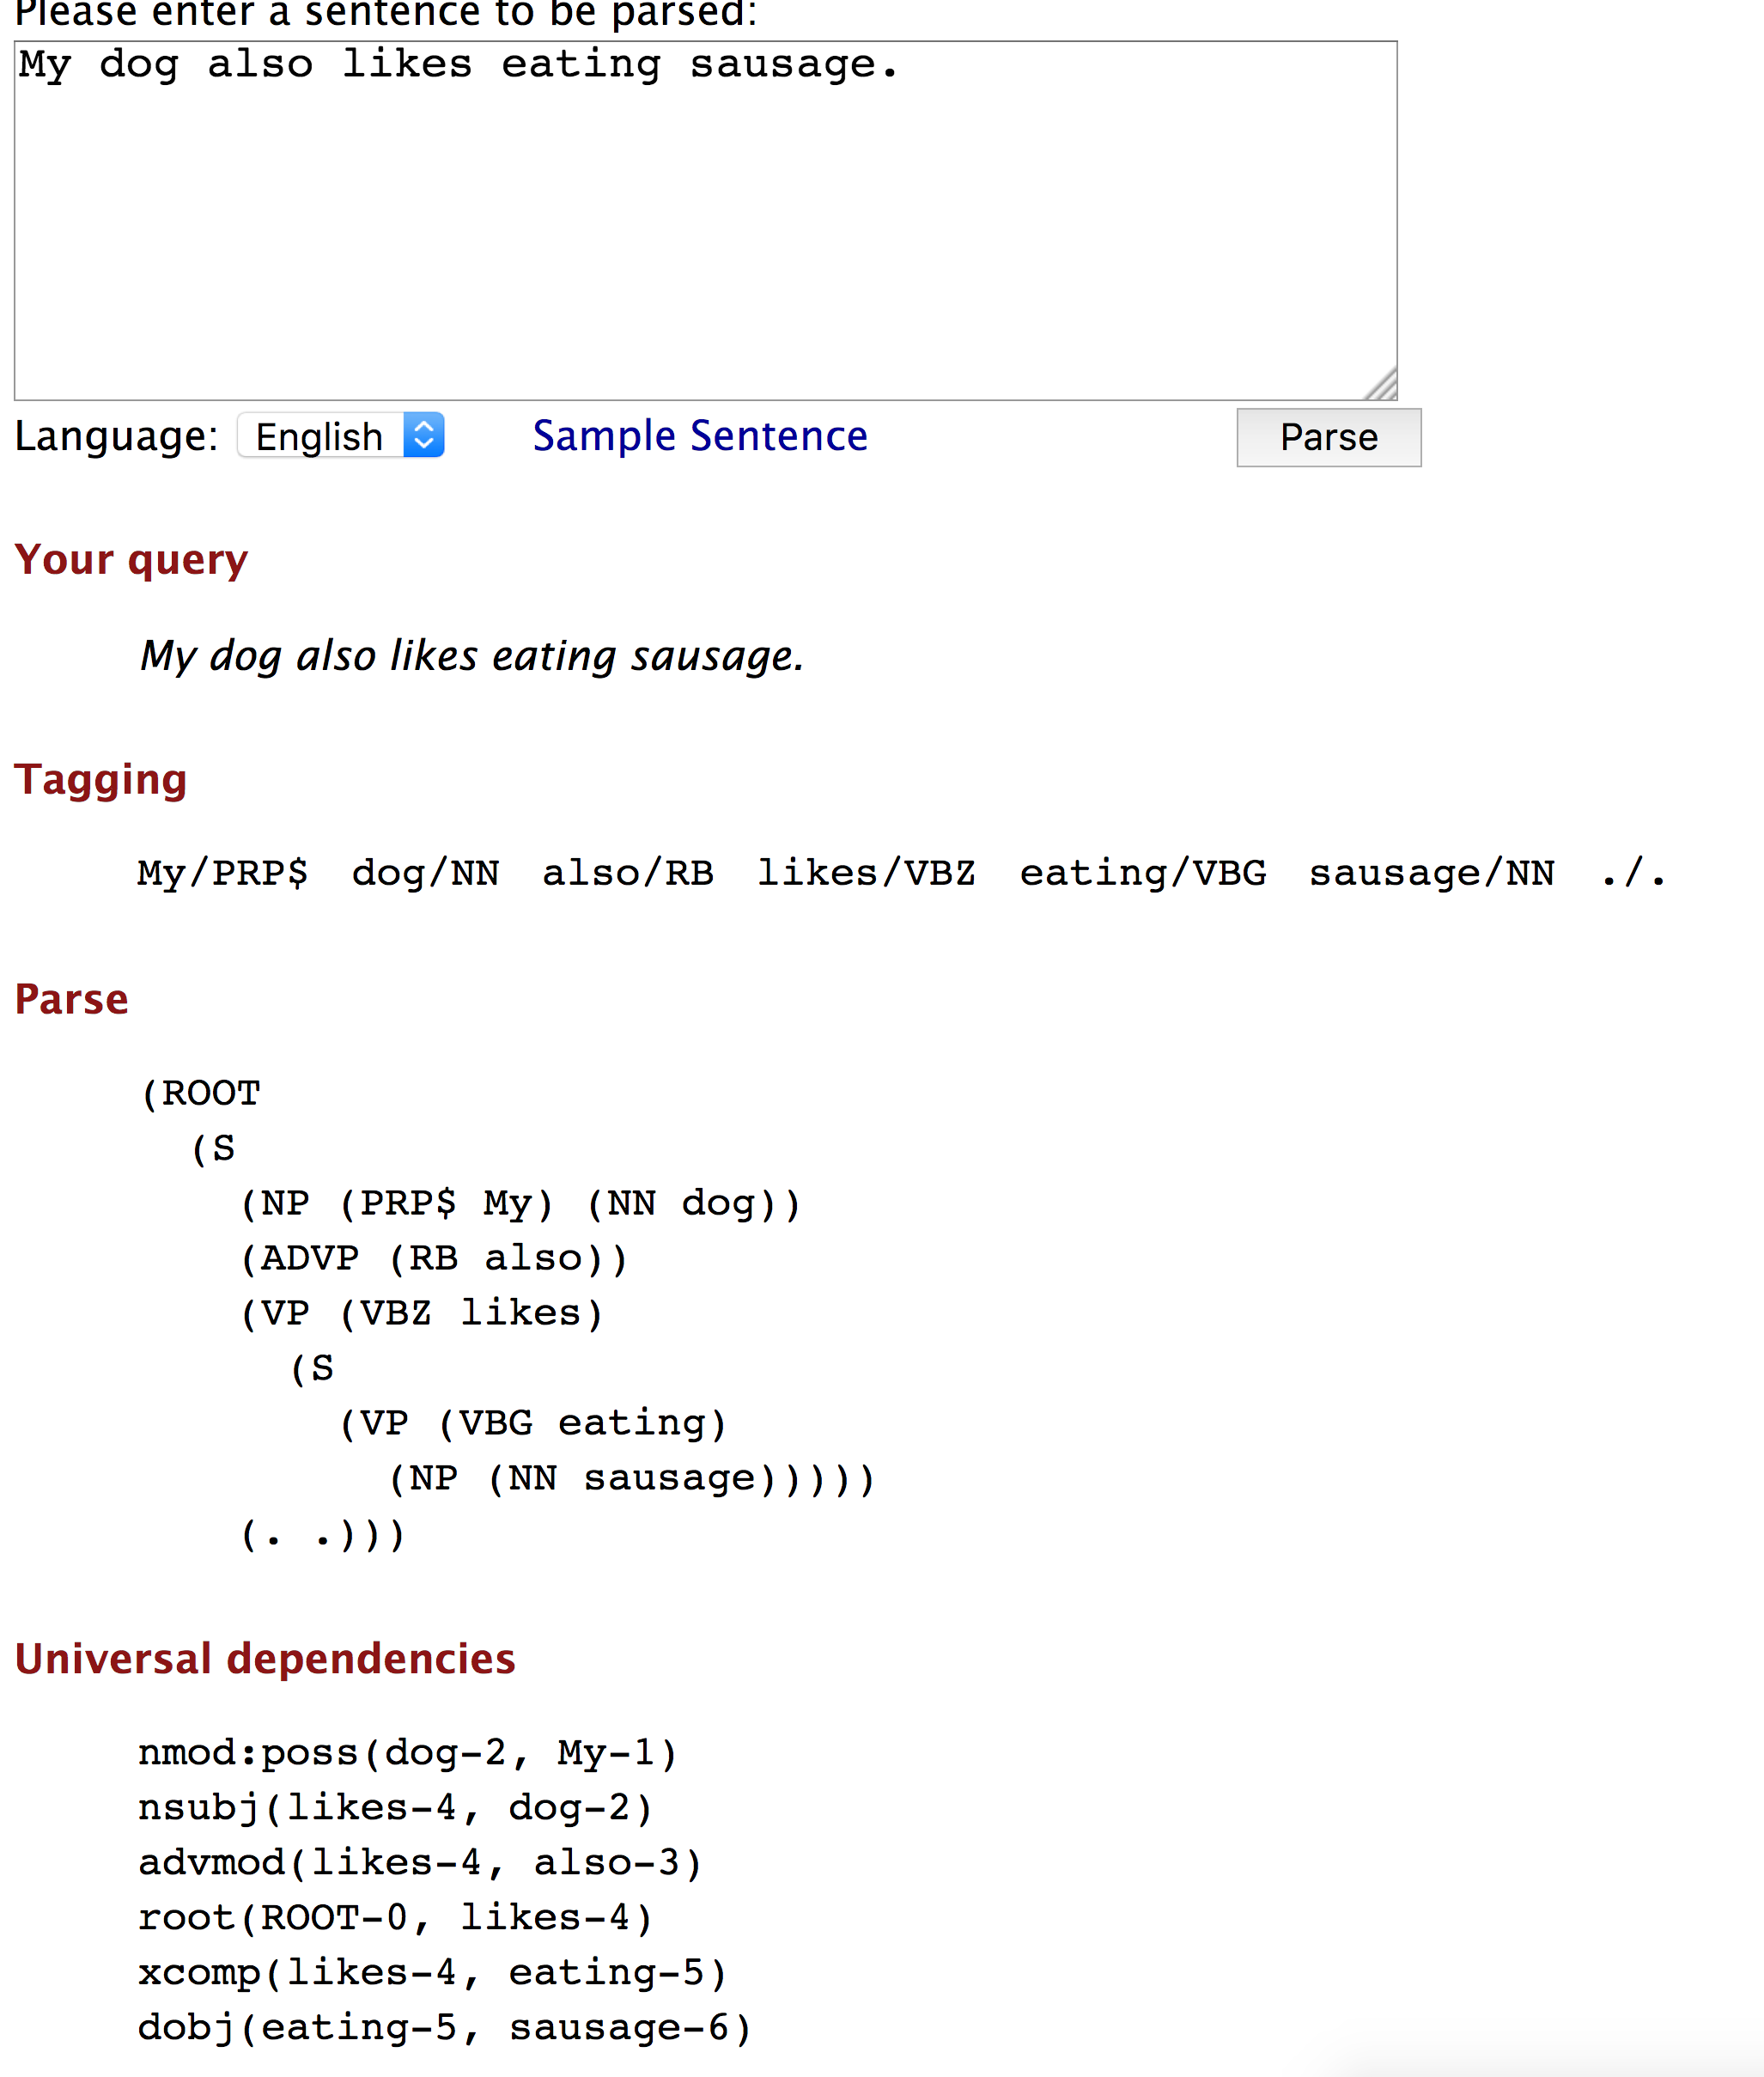
\includegraphics[width=0.6\textwidth]{parses-examples.png}
\end{frame}

\begin{frame}
\frametitle{Constituency Structure: Context Free Grammars}
\begin{itemize}
\item CFG is a mathematical way to model constituent structure in a language. 
\item A CFG consists of:
\begin{enumerate}
\item a set of symbols in the language (lexicon)
\item a set of rules or productions which describe how symbols in that language can be grouped together
\end{enumerate} \pause
\item Example symbols: NP, VP, PP, DT, NN, the, car etc.
\item Example rules: S $->$ NP VP; $->$ DT N; Noun $->$ car etc.
\item Symbols in CFGs are of two types: terminals (words) and non-terminals (NP, N etc)
\end{itemize}
\end{frame}

\begin{frame}
\frametitle{Context Free Grammars - Purpose}
\begin{enumerate}
\item To assign structure to a given sentence
\item To generate sentences automatically
\end{enumerate}
\end{frame}

\begin{frame}
\frametitle{CFG Parsing in NLP: brief history}
\begin{itemize}
\item Compile a grammar (rules), have a lexicon, and use both to derive parses for sentences.
\item Problem: low coverage (all constructions cannot be covered), combinations of rules can create several parses - what is the best parse?
\item 90s: growth of annotated data such as Penn Tree Bank, which resulted in the development of statistical parsers.
\end{itemize}
\end{frame}

\begin{frame}
\frametitle{Constituency structure - Example}
\begin{itemize}
\item Let us say this is my grammar and lexicon together:
\begin{enumerate}
\item S $->$ NP VP (Sentence contains Noun Phrase, Verb Phrase)
\item  VP $->$ V NP $|$ V NP PP $|$ V S $|$ V ADJ ($|$ is or like in regex)
\item PP $->$ P NP
\item V $->$ "saw" $|$ "ate" $|$ "walked"
\item  NP $->$ "John" $|$ "Mary" $|$ "Bob" $|$ Det N $|$ Det N PP $|$ PropN 
 \item Det -$->$ "a" $|$ "an" $|$"the" $|$ "my"
 \item N $->$ "man" $|$ "dog" $|$ "cat" $|$ "telescope" $|$ "park"
 \item P $->$ "in" $|$ "on" $|$ "by" $|$ "with"
\end{enumerate}
\item What will the constituency structure (or phrase structure tree) look like for the sentence: "John saw a man with the telescope"?
\end{itemize}
\end{frame}

\begin{frame}
\frametitle{Recursion in CFGs}
\framesubtitle{Source: NLTK book, Chapter 8}
Note: CFGs can be recursive (What does that mean??) \\
\pause 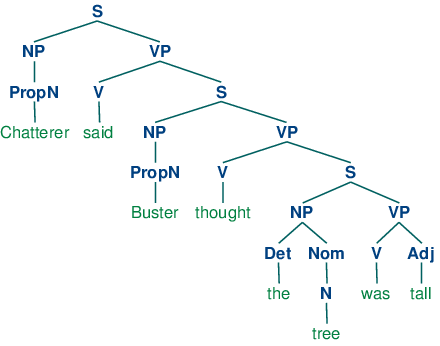
\includegraphics[width=0.9\textwidth]{nltk-tree-example.png}
\end{frame}

\begin{frame}
\frametitle{CFG Parsing in NLP: key issues}
\begin{itemize}
\item Attachment ambiguities: where to attach a PP, a conjunction etc. 
\item Two problems arise due to this:
\begin{enumerate}
\item You should explore multiple parses and pick the most likely one. 
\item In this process, there are many sub-processes that repeat, and we should somehow preserve this information to not start from scratch for each possibility.
\end{enumerate}
\end{itemize}
\end{frame}

\begin{frame}
\frametitle{CFG Parsing in NLP: key issues}
\framesubtitle{Source: Jurafsky and Manning's Coursera lectures}
For a sentence: cats scratch people with cats with claws.
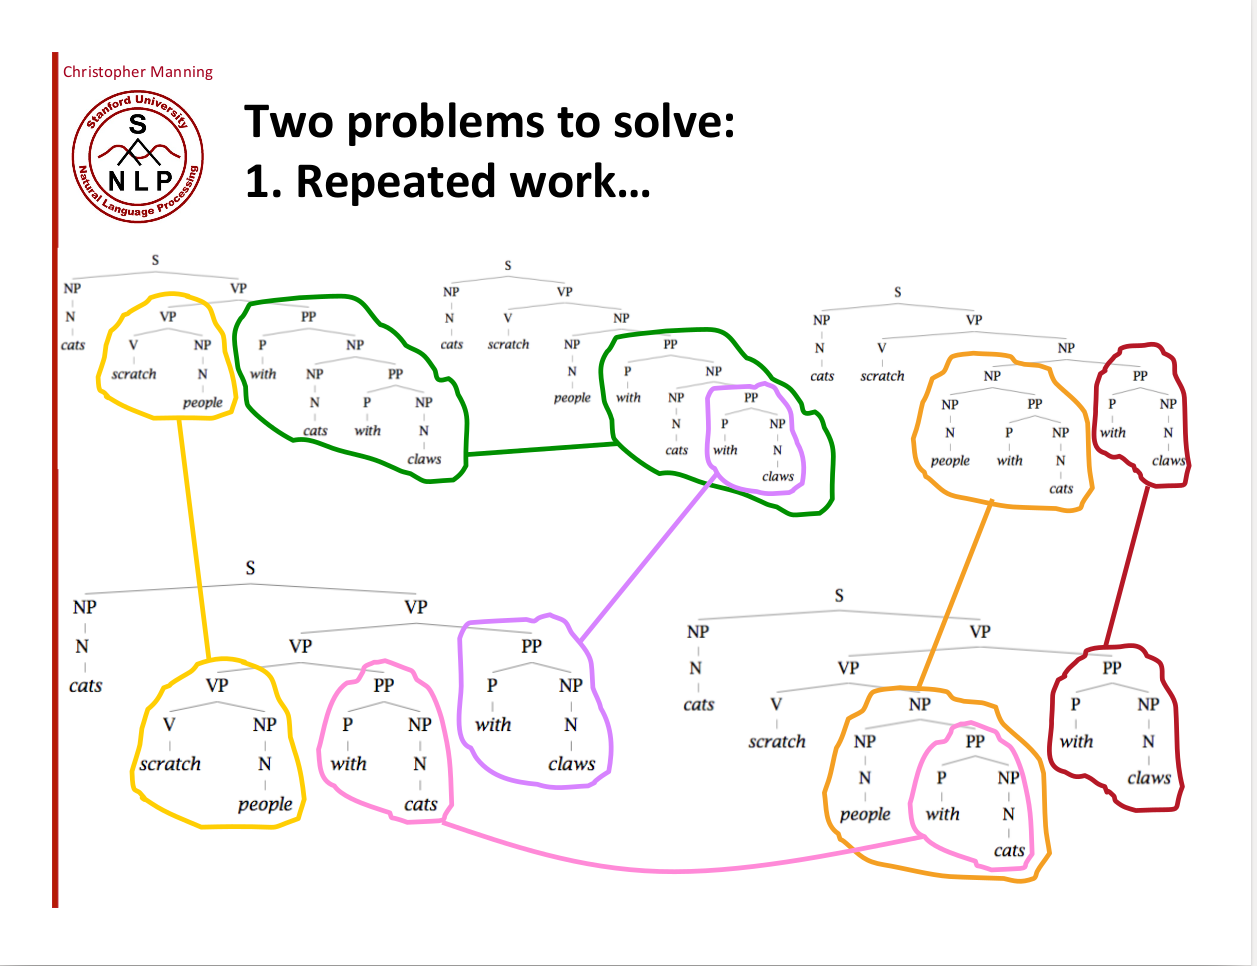
\includegraphics[width=0.9\textwidth]{parsing.png}
\end{frame}

\begin{frame}
\frametitle{CFG Parsing: Methods}
\begin{itemize}
\item Recursive Descent Parsing (Top-down)
\item Shift Reduce parsing (bottom up)
\item left-corner parsing
\item chart parsing
\item ...
\end{itemize}
.. overview on Tuesday.
\end{frame}

\begin{frame}
\frametitle{Probabilistic CFG Parsing}
\framesubtitle{Source: Jurafsky and Manning's Coursera lectures}
Relies on treebank data to get these probabilities for each rule.
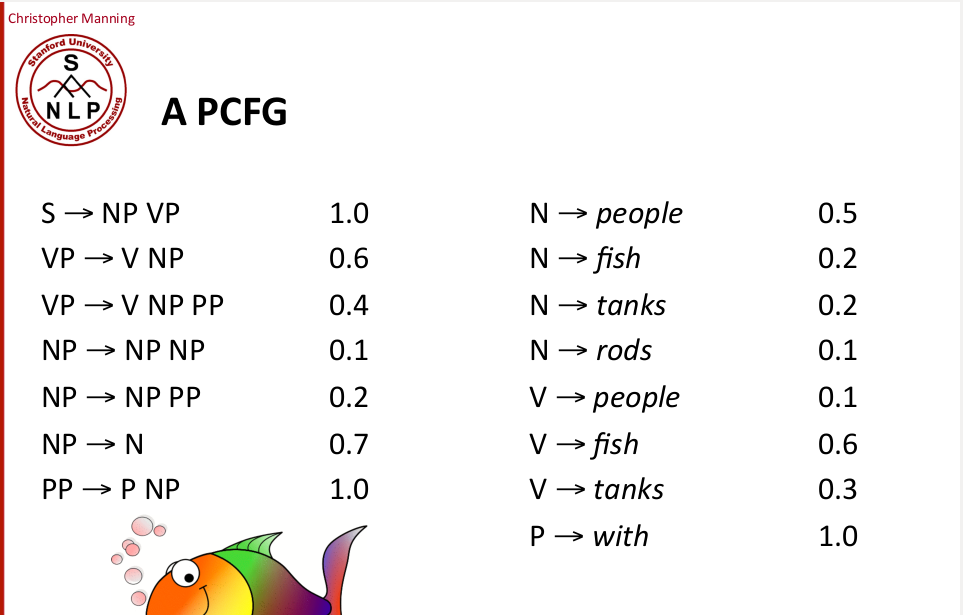
\includegraphics[width=0.9\textwidth]{pcfg.png}
\end{frame}

\begin{frame}
\frametitle{Exercise -1}
\framesubtitle{Source: Exercise 12.2 in J\&M}
Draw tree structures for the following sentences, after creating a grammar together.
\begin{itemize}
\item I would like to fly on American airlines.
\item Please repeat that.
\item Does American 487 have a first class section?
\item I need to fly between Philadelphia and Atlanta
\item Does American airlines have a flight between five a.m. and six a.m.?
\item What is the fare from Atlanta to Denver?
\item Is there an American airlines flight from Philadelphia to Dallas?
\end{itemize}
\end{frame}

\begin{frame}
\frametitle{Exercise-2: NLTK}
\framesubtitle{Source: Chapter 8 in NLTK Book}
\begin{enumerate}
\item Follow the groucho grammar example in Section 1.2 and simple grammar example in Section 3.1 that uses recursive descent parser.
\item After that, use the grammar in Section 3.3 instead of groucho grammar, and try to parse examples 10 (a) and (b) in the textbook with this grammar.
\item Finally: Figure out how to make Example 3.2 work on your computer, with your own custom created grammar.
\end{enumerate}
\end{frame}

\begin{frame}
\frametitle{Another Exercise}
Figure out how to use Stanford parser in NLTK. I will ask about this in Tuesday's class. Work outside the class if needed and find a solution.
\end{frame}

\begin{frame}
\frametitle{Next Week}
\begin{enumerate}
\item Topics: 
\begin{itemize}
\item CFG parsing algorithms overview
\item Dependency grammars
\item using dependency parsers in NLTK
\item Constituency vs Dependency parsing - which is more useful and when?
\end{itemize}
\item Readings: Chapter 8 in NLTK (Mandatory). Chapter 12--14 in J\&M (Optional)
\item Video lectures (optional): Week 5 Lectures in Jurafsky and Manning's course or Weeks 4 and 5 lectures in Radev's course.
\end{enumerate}
\end{frame}
\end{document}


Next week:
%Chunking

%How is a CFG based parsing done?
%attachment ambiguities, exponential possibilities, example
%how to handle these. 

%NLTK practice.

\begin{frame}
\frametitle{Dependency Structure - Example}
\begin{itemize}
\item Let us ignore what exactly are the names of relations for a moment, and look at the same sentence from previous slide.
\item How can we show dependency relations between words instead of phrase structure relations?
\end{itemize}
\end{frame}




\begin{frame}
\frametitle{Programming exercise - 1}
\begin{itemize}
\item Take any .txt version file from gutenberg.org, written by your favorite author (in English!)
\item Read that file into your python code, and do the following using NLTK:
\begin{enumerate}
\item Split the file into sentences.
\item Print the following: number of sentences in the file, average sentence length (in number of words), average word length (in number of characters), number of unique words, number of unique stems.
\item Note 1: Once sentence splitting is done, you can ignore punctuation markers for the rest of the calculation.
\item Note 2: You can use any stemmer you want.
\end{enumerate}
\end{itemize}
\end{frame}

\begin{frame}
\frametitle{Programming exercise - 1}
\begin{itemize}
\item For the same file from last slide, do the following:
\item Read that file into your python code, and do the following using NLTK:
\begin{enumerate}
\item Split the file into sentences.
\item For each sentence, print its POS tagged version as a string of tags. E.g., if you have "It is a sentence" as your sentence, and your NLTK tagger outputs the tags for this sentence as a list (or tuple or whatever), you should print the tag as a string. E.g., PRP VBZ DT NN (not as [PRP, VBZ, DT, NN] or as [(It, PRP), (is, VBZ) .. ... ])
\end{enumerate}
\end{itemize}
\end{frame}
